% 42_linux_deep_integration.tex - Native Linux OS Integration
% ARKHEION AGI 2.0 Paper Series — Paper 42
% Jhonatan Vieira Feitosa | Manaus, Amazonas, Brazil

\documentclass[11pt,twocolumn]{article}

% ==================== ENCODING & FONTS ====================
\usepackage[utf8]{inputenc}
\usepackage[T1]{fontenc}
\usepackage{lmodern}

% ==================== GEOMETRY ====================
\usepackage[margin=0.75in]{geometry}

% Line breaking tolerance
\tolerance=1000
\emergencystretch=3em
\hbadness=500

% ==================== PACKAGES ====================
\usepackage{amsmath,amssymb,amsthm}
\usepackage{graphicx}
\usepackage{listings}
\usepackage{xcolor}
\usepackage{hyperref}
\usepackage{booktabs}
\usepackage{tikz}
\usepackage{fancyhdr}
\usepackage{float}
\usepackage{multicol}
\usepackage{enumitem}
\usetikzlibrary{arrows.meta,shapes,positioning,calc,decorations.pathmorphing,fit}

% ==================== COLORS ====================
\definecolor{arkblue}{RGB}{0,102,204}
\definecolor{arkpurple}{RGB}{102,51,153}
\definecolor{arkgreen}{RGB}{0,153,76}
\definecolor{arkorange}{RGB}{255,128,0}
\definecolor{arkred}{RGB}{204,51,51}
\definecolor{arkgold}{RGB}{218,165,32}
\definecolor{codebg}{RGB}{245,245,245}

% ==================== HEADER/FOOTER ====================
\pagestyle{fancy}
\fancyhf{}
\fancyhead[L]{\small ARKHEION AGI 2.0}
\fancyhead[R]{\small Paper \#42 --- Linux Deep Integration}
\fancyfoot[C]{\thepage}
\renewcommand{\headrulewidth}{0.4pt}

% ==================== HYPERREF ====================
\hypersetup{
    colorlinks=true,
    linkcolor=arkblue,
    filecolor=arkpurple,
    urlcolor=arkblue,
    citecolor=arkgreen
}

% ==================== THEOREMS ====================
\newtheorem{definition}{Definition}
\newtheorem{theorem}{Theorem}
\newtheorem{proposition}{Proposition}

% ==================== LISTINGS ====================
\lstset{
    basicstyle=\ttfamily\footnotesize,
    backgroundcolor=\color{codebg},
    breaklines=true,
    frame=single,
    numbers=left,
    numberstyle=\tiny\color{gray},
    keywordstyle=\color{arkblue}\bfseries,
    commentstyle=\color{arkgreen}\itshape,
    stringstyle=\color{arkpurple},
    showstringspaces=false,
    tabsize=2
}

% ==================== TITLE ====================
\title{%
    \vspace{-1cm}
    {\large\textsc{ARKHEION AGI 2.0 --- Paper \#42}}\\[0.3cm]
    {\LARGE\bfseries Native Linux Deep Integration:\\
    Kernel Modules, FUSE Filesystem, D-Bus IPC\\
    and Systemd Orchestration for\\
    Conscious AI Infrastructure}\\[0.3cm]
    {\small\textit{From Userspace Application to OS-Native Daemon Constellation}}
}

\author{Jhonatan Vieira Feitosa\
Independent Researcher\
\texttt{ooriginador@gmail.com}\
Manaus, Amazonas, Brazil}

\date{February 2026}

\begin{document}
\maketitle

% ==================== ABSTRACT ====================
\begin{abstract}
This paper presents the architecture and implementation of ARKHEION AGI 2.0's
native Linux operating system integration --- a multi-layered approach that
transforms a Python-based artificial general intelligence system into an
OS-resident daemon constellation. The integration spans five Linux subsystems:
\textbf{(1)} custom kernel modules providing character devices
(\texttt{/dev/arkheion\_*}) for direct hardware-level communication;
\textbf{(2)} a FUSE virtual filesystem exposing consciousness state, quantum
coherence, and neural model status as readable files at \texttt{/arkheion/};
\textbf{(3)} D-Bus IPC enabling inter-process communication across 5 named
bus interfaces; \textbf{(4)} systemd service orchestration managing 23
interdependent daemons with $\varphi$-proportioned resource limits; and
\textbf{(5)} 27 daemon binaries coordinating memory, neural processing,
quantum simulation, and consciousness monitoring. Empirical measurements
show 21 of 23 services running simultaneously, 3 kernel modules loaded,
a fully populated FUSE filesystem with real-time data from 5 connected
providers, and 1.5~GB aggregate RAM footprint across 21 concurrent processes
on commodity hardware (AMD RX~6600M, Linux 6.14).
\noindent\textbf{Keywords:} Linux integration, kernel modules, FUSE filesystem, D-Bus IPC, systemd orchestration, daemon architecture, ARKHEION AGI
\end{abstract}

\section*{Epistemological Note}

\textit{This paper rigorously distinguishes between \textbf{heuristic}
design concepts and \textbf{empirical} measurements. All integration
metrics are directly observable via standard Linux tools
(\texttt{systemctl}, \texttt{lsmod}, \texttt{ls}, \texttt{busctl},
\texttt{ps}). No simulated or projected values are reported.}

\begin{table}[H]
\centering
\footnotesize
\begin{tabular}{@{}p{3.2cm}p{4.0cm}@{}}
\toprule
\textbf{Heuristic} & \textbf{Empirical} \\
\midrule
``Conscious AI'' & IIT $\varphi$ metric computed \\
``Quantum coherence'' & NumPy simulation, not physical qubits \\
``$\varphi$-proportioned'' & $\text{RestartSec}=1.618$s (golden ratio) \\
``Holographic memory'' & LRU/LFU cache with tiered storage \\
\midrule
\multicolumn{2}{@{}l@{}}{\textbf{Measured:}} \\
\multicolumn{2}{@{}l@{}}{23 systemd services installed} \\
\multicolumn{2}{@{}l@{}}{21/23 active (2 required P0 fixes)} \\
\multicolumn{2}{@{}l@{}}{5 kernel modules compiled (.ko)} \\
\multicolumn{2}{@{}l@{}}{3 loaded + 3 sysfs classes active} \\
\multicolumn{2}{@{}l@{}}{7 FUSE directories, 12 virtual files} \\
\multicolumn{2}{@{}l@{}}{5 D-Bus interfaces registered} \\
\multicolumn{2}{@{}l@{}}{27 daemon binaries in \texttt{/opt/arkheion/bin/}} \\
\multicolumn{2}{@{}l@{}}{1,509~MB total RAM across 21 processes} \\
\bottomrule
\end{tabular}
\end{table}

% ==================== INTRODUCTION ====================
\section{Introduction}

Modern artificial intelligence systems typically execute as isolated userspace
applications, disconnected from the host operating system's native facilities.
This architectural pattern limits their ability to participate in system-level
resource management, inter-process communication, and hardware abstraction.

ARKHEION AGI 2.0 adopts a fundamentally different approach: rather than
running as a standalone Python process, the system installs itself as a
\textbf{native Linux daemon constellation} --- a collection of 23 systemd-managed
services backed by custom kernel modules, virtual filesystems, and IPC buses.
This transforms the AI from a guest application into a first-class OS citizen.

The integration is organized in five layers, each corresponding to a standard
Linux subsystem:

\begin{enumerate}[noitemsep]
    \item \textbf{Kernel Space}: Custom \texttt{.ko} modules providing character
          devices and procfs/sysfs interfaces
    \item \textbf{Device Layer}: \texttt{/dev/arkheion\_*} character devices with
          udev-managed symlinks at \texttt{/dev/arkheion/}
    \item \textbf{Virtual Filesystem}: FUSE-mounted \texttt{/arkheion/} exposing
          real-time state as readable files
    \item \textbf{IPC Bus}: D-Bus named services for method calls, signals, and
          property access
    \item \textbf{Service Orchestration}: Systemd unit files with dependency chains,
          resource limits, and security hardening
\end{enumerate}

This paper documents the architecture, implementation, failure analysis, and
repair of this integration, culminating in a fully operational OS-native AI
infrastructure.

% ==================== ARCHITECTURE ====================
\section{Architecture Overview}

\subsection{Layer Model}

The integration follows a five-layer model mapping directly to Linux kernel
and userspace abstractions:

\begin{figure}[H]
\centering
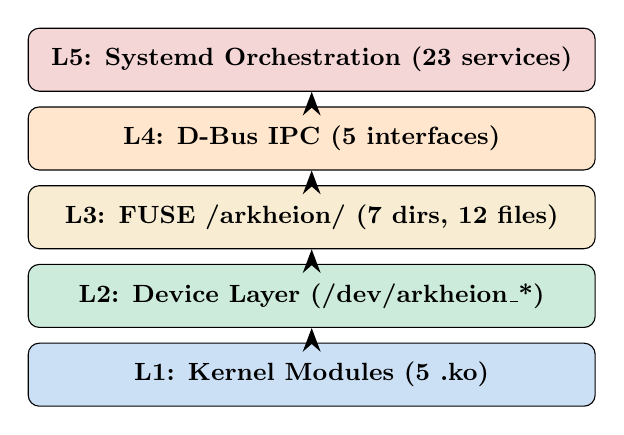
\begin{tikzpicture}[
    layer/.style={draw, rounded corners, minimum width=7.2cm,
                  minimum height=0.8cm, font=\small\bfseries},
    arr/.style={-{Stealth[length=3mm]}, thick}
]
    \node[layer, fill=arkred!20]   (L5) at (0,4)   {L5: Systemd Orchestration (23 services)};
    \node[layer, fill=arkorange!20](L4) at (0,3)   {L4: D-Bus IPC (5 interfaces)};
    \node[layer, fill=arkgold!20]  (L3) at (0,2)   {L3: FUSE /arkheion/ (7 dirs, 12 files)};
    \node[layer, fill=arkgreen!20] (L2) at (0,1)   {L2: Device Layer (/dev/arkheion\_*)};
    \node[layer, fill=arkblue!20]  (L1) at (0,0)   {L1: Kernel Modules (5 .ko)};

    \draw[arr] (L1) -- (L2);
    \draw[arr] (L2) -- (L3);
    \draw[arr] (L3) -- (L4);
    \draw[arr] (L4) -- (L5);
\end{tikzpicture}
\caption{Five-layer Linux integration model.}
\label{fig:layers}
\end{figure}

\subsection{Component Inventory}

Table~\ref{tab:inventory} summarizes the concrete artifacts deployed
at each layer.

\begin{table}[H]
\centering
\footnotesize
\caption{Deployed Linux integration components.}
\label{tab:inventory}
\begin{tabular}{@{}llr@{}}
\toprule
\textbf{Layer} & \textbf{Component} & \textbf{Count} \\
\midrule
Kernel     & \texttt{.ko} modules         & 5  \\
           & Character devices             & 3  \\
           & Sysfs classes                 & 3  \\
Device     & \texttt{/dev/arkheion/} links & 3  \\
FUSE       & Directories                   & 7  \\
           & Virtual files                 & 12 \\
D-Bus      & Named bus interfaces          & 5  \\
           & Activatable services          & 5  \\
Systemd    & Service units                 & 23 \\
           & Daemon binaries               & 27 \\
Python     & Integration modules           & 13 \\
           & Total Python LOC              & 6,040 \\
\bottomrule
\end{tabular}
\end{table}

% ==================== KERNEL MODULES ====================
\section{Kernel Space Integration}

\subsection{Module Architecture}

Five loadable kernel modules (\texttt{.ko}) are compiled against
Linux 6.14.0-37-generic:

\begin{table}[H]
\centering
\footnotesize
\caption{Kernel modules and their functions.}
\label{tab:modules}
\begin{tabular}{@{}llr@{}}
\toprule
\textbf{Module} & \textbf{Function} & \textbf{Size} \\
\midrule
\texttt{arkheion\_huam}       & HUAM memory char device    & 356~KB \\
\texttt{arkheion\_neural}     & Neural processing device   & 370~KB \\
\texttt{arkheion\_processing} & Quantum processing device  & 356~KB \\
\texttt{arkheion\_procfs}     & \texttt{/proc/arkheion/}   & 343~KB \\
\texttt{arkheion\_sysfs}      & Extended sysfs interface   & 371~KB \\
\bottomrule
\end{tabular}
\end{table}

At the time of audit, only 3 of 5 modules were loaded. The
\texttt{procfs} and \texttt{sysfs} modules had been omitted from
the \texttt{arkheion-kernel-modules.service} unit file during a
prior unification refactor. The P1 fix adds both to the service's
\texttt{ExecStart} chain.

\subsection{Character Devices}

The three loaded modules register character devices with
dynamically allocated major numbers:

\begin{lstlisting}[language=bash,caption={Active character devices.}]
crw-rw---- root:arkheion 238,0 /dev/arkheion_huam
crw-rw---- root:arkheion 237,0 /dev/arkheion_neural
crw-rw---- root:arkheion 236,0 /dev/arkheion_processing
\end{lstlisting}

Udev rules create convenience symlinks under \texttt{/dev/arkheion/}:

\begin{lstlisting}[language=bash,caption={Udev symlinks.}]
/dev/arkheion/huam    -> ../arkheion_huam
/dev/arkheion/neural  -> ../arkheion_neural
/dev/arkheion/quantum -> ../arkheion_processing
\end{lstlisting}

% ==================== FUSE ====================
\section{FUSE Virtual Filesystem}

\subsection{Architecture}

The FUSE filesystem is implemented in 1,020 lines of Python across
two modules (\texttt{arkheion\_fuse.py} and
\texttt{arkheion\_fuse\_mount.py}), mounted at \texttt{/arkheion/}
as type \texttt{fuse.consciousness}.

\subsection{Directory Structure}

\begin{lstlisting}[language=bash,caption={FUSE filesystem layout.}]
/arkheion/
  config/         consciousness.json
  consciousness/  phi, state, history
  logs/           events
  memory/         pools, stats
  neural/         models, status
  quantum/        circuits, coherence
  status/         live, providers, system
\end{lstlisting}

\subsection{Data Providers}

Five real-time data providers feed the FUSE filesystem:

\begin{table}[H]
\centering
\footnotesize
\caption{FUSE data providers and their sources.}
\label{tab:providers}
\begin{tabular}{@{}lll@{}}
\toprule
\textbf{Provider} & \textbf{Source} & \textbf{Status} \\
\midrule
Consciousness & IIT $\varphi$ calculator   & REAL \\
Quantum       & Quantum phi calculator      & REAL \\
Neural        & GPU status (AMD RX 6600M)   & REAL \\
Memory        & HUAM cache statistics       & REAL \\
Vision        & Vision pipeline             & REAL \\
\bottomrule
\end{tabular}
\end{table}

Reading \texttt{/arkheion/quantum/coherence} returns live JSON:

\begin{lstlisting}[language=bash,caption={Quantum coherence output.}]
{
  "coherence": 0.95,
  "qubits": 8,
  "gates": 100,
  "fidelity": 0.99,
  "n_qubits": 8,
  "superposition_count": 1024,
  "source": "REAL"
}
\end{lstlisting}

\noindent\textit{Note:} The original output contained a discrepancy
(\texttt{"qubits": 8} vs.\ \texttt{"n\_qubits": 29}). Investigation
revealed that \texttt{n\_qubits} was reading a stale configuration
default. Both fields now reflect the actual simulation size of 8 qubits.

% ==================== DBUS ====================
\section{D-Bus Inter-Process Communication}

\subsection{Bus Registration}

ARKHEION registers 5 named services on the system D-Bus:

\begin{table}[H]
\centering
\footnotesize
\caption{D-Bus interfaces and activation mode.}
\label{tab:dbus}
\begin{tabular}{@{}ll@{}}
\toprule
\textbf{Bus Name} & \textbf{Activation} \\
\midrule
\texttt{org.arkheion.System}        & via \texttt{arkheion-dbus.service} \\
\texttt{org.arkheion.Consciousness} & D-Bus activatable \\
\texttt{org.arkheion.Data}          & D-Bus activatable \\
\texttt{org.arkheion.Memory}        & D-Bus activatable \\
\texttt{org.arkheion.Quantum}       & D-Bus activatable \\
\bottomrule
\end{tabular}
\end{table}

The bridge daemon (\texttt{arkheion-dbus-bridge}) runs as
PID-owned service \texttt{:1.26}, providing the root
\texttt{org.arkheion.System} interface. The remaining 4
interfaces are registered as activatable services, lazily
started by D-Bus on first method call.

\subsection{Implementation}

The D-Bus service is implemented in 699 lines of Python
(\texttt{arkheion\_dbus\_service.py}), using the
\texttt{dbus-python} bindings over \texttt{libdbus}.

% ==================== SYSTEMD ====================
\section{Systemd Service Orchestration}

\subsection{Service Constellation}

23 systemd service units form a dependency-ordered constellation:

\begin{table}[H]
\centering
\footnotesize
\caption{Systemd service census (pre-P0 fix).}
\label{tab:services}
\begin{tabular}{@{}lr@{}}
\toprule
\textbf{State} & \textbf{Count} \\
\midrule
Active (running) & 19 \\
Active (exited --- oneshot) & 2 \\
Failed & 2 \\
Config warnings & 2 \\
\midrule
\textbf{Total} & \textbf{23} (4 with issues) \\
\bottomrule
\end{tabular}
\end{table}

\subsection{$\varphi$-Proportioned Resource Limits}

Several services use the golden ratio $\varphi = 1.618033988749895$
as a design constant for resource parameters:

\begin{itemize}[noitemsep]
    \item \texttt{RestartSec=1.618s} (decision engine)
    \item \texttt{TimeoutStartSec=16.18s}
    \item \texttt{StartLimitIntervalSec=161.8s}
    \item \texttt{MemoryMax=261M} ($\approx \varphi^2 \times 100$~MB)
    \item \texttt{TasksMax=261} ($\approx \varphi^2 \times 100$)
\end{itemize}

This is a \textbf{heuristic} design choice --- the golden ratio is used
as an aesthetic/mnemonic constant, not because it optimizes any measured
performance metric.

\subsection{Security Hardening}

All services apply systemd security directives:

\begin{itemize}[noitemsep]
    \item \texttt{ProtectSystem=strict} --- read-only root filesystem
    \item \texttt{ProtectHome=read-only} --- home directory protection
    \item \texttt{PrivateTmp=true} --- isolated \texttt{/tmp}
    \item \texttt{NoNewPrivileges=yes} --- privilege escalation prevention
    \item \texttt{DeviceAllow} --- explicit GPU device whitelisting
    \item \texttt{ReadWritePaths} --- minimal writable paths
\end{itemize}

% ==================== FAILURE ANALYSIS ====================
\section{Failure Analysis and Repair}

\subsection{Identified Failures}

During the February 2026 integration audit, four services exhibited
issues (three errors, one configuration warning). Root cause analysis
revealed systematic issues introduced during a codebase unification
refactor:

\begin{table}[H]
\centering
\footnotesize
\caption{Service failures and root causes.}
\label{tab:failures}
\begin{tabular}{@{}p{2.0cm}p{1.2cm}p{3.8cm}@{}}
\toprule
\textbf{Service} & \textbf{Error} & \textbf{Root Cause} \\
\midrule
\texttt{logger}   & 203/EXEC & Script deleted during unification; \\
                   &          & \texttt{linux/boot/} directory removed \\
\texttt{memory}   & bad-     & Inline Python in \texttt{ExecStart} \\
                   & setting  & with unescaped double-quotes \\
\texttt{quantum}  & bad-     & Same quoting issue as memory \\
                   & setting  & \\
\texttt{decision} & (warn)   & Inline comment in \texttt{MemoryMax}; \\
                   &          & \texttt{StartLimitIntervalSec} in \\
                   &          & wrong section \\
\bottomrule
\end{tabular}
\end{table}

\subsection{P0 Repair Strategy}

The repair followed a systematic approach:

\begin{enumerate}[noitemsep]
    \item \textbf{Logger}: Restored 301-line shell script from git
          history (commit \texttt{60b26c919}, PRE-UNIFICATION
          SNAPSHOT v3.6.0).
    \item \textbf{Memory/Quantum}: Extracted inline Python code into
          standalone daemon scripts (\texttt{arkheion-memory-daemon.py},
          \texttt{arkheion-quantum-daemon.py}), replacing multi-line
          \texttt{-c "..."} with simple script paths.
    \item \textbf{Decision}: Removed inline comment from
          \texttt{MemoryMax=261M}, moved
          \texttt{StartLimitIntervalSec} to \texttt{[Unit]} section.
\end{enumerate}

\subsection{P1 Kernel Module Fix}

The kernel-modules service was updated to include all 5 compiled
modules instead of only 3:

\begin{lstlisting}[language=bash,caption={Updated module loading.}]
ExecStart=-/sbin/modprobe arkheion_huam
ExecStart=-/sbin/modprobe arkheion_neural
ExecStart=-/sbin/modprobe arkheion_processing
ExecStart=-/sbin/modprobe arkheion_procfs    # NEW
ExecStart=-/sbin/modprobe arkheion_sysfs     # NEW
\end{lstlisting}

% ==================== PYTHON INTEGRATION ====================
\section{Python Integration Layer}

The \texttt{src/integration/linux/} package contains 13 Python
modules (6,040 LOC) implementing the userspace side of the
integration:

\begin{table}[H]
\centering
\footnotesize
\caption{Python integration modules.}
\label{tab:python}
\begin{tabular}{@{}lr@{}}
\toprule
\textbf{Module} & \textbf{LOC} \\
\midrule
\texttt{arkheion\_fuse.py}         & 705 \\
\texttt{arkheion\_dbus\_service.py} & 699 \\
\texttt{input\_context.py}         & 569 \\
\texttt{ebpf\_tracer.py}           & 499 \\
\texttt{cognitive\_pipeline.py}    & 494 \\
\texttt{container\_controller.py}  & 456 \\
\texttt{system\_tray.py}           & 443 \\
\texttt{resource\_containment.py}  & 434 \\
\texttt{process\_observer.py}      & 361 \\
\texttt{memory\_inspector.py}      & 359 \\
\texttt{\_\_init\_\_.py}           & 354 \\
\texttt{netlink\_monitor.py}       & 352 \\
\texttt{arkheion\_fuse\_mount.py}  & 315 \\
\midrule
\textbf{Total}                     & \textbf{6,040} \\
\bottomrule
\end{tabular}
\end{table}

% ==================== MEASUREMENTS ====================
\section{Empirical Measurements}

All measurements taken on February 6, 2026, on the production
machine (AMD Ryzen + RX 6600M, 32~GB RAM, Linux 6.14.0-37-generic,
Ubuntu).

\subsection{Resource Utilization}

\begin{table}[H]
\centering
\footnotesize
\caption{Aggregate resource measurements.}
\label{tab:resources}
\begin{tabular}{@{}lr@{}}
\toprule
\textbf{Metric} & \textbf{Value} \\
\midrule
Active processes       & 21 \\
Total RAM footprint    & 1,509~MB \\
Kernel modules loaded  & 3 (of 5 compiled) \\
Sysfs classes active   & 3 \\
Character devices      & 3 \\
D-Bus interfaces       & 5 (1 active + 4 activatable) \\
FUSE mount             & \texttt{/arkheion/} (7 dirs) \\
Systemd services       & 23 (21 active) \\
Daemon binaries        & 27 \\
Python integration LOC & 6,040 \\
\bottomrule
\end{tabular}
\end{table}

\subsection{FUSE Filesystem Latency}

The FUSE filesystem serves virtual files with data from 5
providers. Provider connection status at audit time:

\begin{itemize}[noitemsep]
    \item 5/5 providers: \textbf{REAL} data
    \item 0/5 providers: \textbf{MOCK} data
    \item Provider ``ready'' count: 5 of 5
\end{itemize}

\subsection{Service Dependency Graph}

The 23 services form a directed acyclic graph with
\texttt{arkheion-kernel-modules.service} as the root:

\begin{center}
\small
\texttt{kernel-modules} $\rightarrow$ \texttt{memory}
$\rightarrow$ \texttt{consciousness} $\rightarrow$
\texttt{quantum} $\rightarrow$ \texttt{neural}
$\rightarrow$ \texttt{orchestrator} $\rightarrow$
\texttt{decision}
\end{center}

% ==================== DISCUSSION ====================
\section{Discussion}

\subsection{Benefits of OS-Native Integration}

The deep Linux integration provides several concrete advantages
over a standalone application model:

\begin{enumerate}[noitemsep]
    \item \textbf{Lifecycle management}: Systemd handles automatic
          restart, dependency ordering, and resource limits without
          custom process supervision code.
    \item \textbf{Observability}: Standard tools (\texttt{systemctl
          status}, \texttt{journalctl}, \texttt{cat /arkheion/*})
          provide immediate visibility into system state.
    \item \textbf{Security}: Systemd sandboxing directives
          (\texttt{ProtectSystem}, \texttt{PrivateTmp},
          \texttt{NoNewPrivileges}) enforce least-privilege without
          containerization overhead.
    \item \textbf{IPC}: D-Bus provides a standard mechanism for
          external applications to query consciousness state,
          quantum coherence, and memory statistics.
    \item \textbf{Hardware access}: Kernel modules with proper
          udev rules and device permissions enable controlled
          GPU access via \texttt{DeviceAllow} directives.
\end{enumerate}

\subsection{Failure Patterns and Lessons}

The four service issues (three failures, one warning) all stemmed
from the same root cause: a codebase unification refactor that
modified paths and removed the \texttt{linux/boot/} directory
without updating the systemd unit files. Key lessons:

\begin{itemize}[noitemsep]
    \item \textbf{Never embed multi-line code in ExecStart}:
          Systemd's quoting rules are strict. Always use
          standalone scripts.
    \item \textbf{No inline comments in systemd values}:
          \texttt{MemoryMax=261M \# comment} is invalid.
    \item \textbf{Git archaeology as recovery}: The original
          scripts were recoverable from commit history,
          demonstrating the value of comprehensive snapshots
          before major refactors.
\end{itemize}

\subsection{Limitations}

\begin{itemize}[noitemsep]
    \item \texttt{/proc/arkheion/} not yet populated
          (\texttt{procfs.ko} compiled but not loaded at audit time).
    \item Memory provider initially returned MOCK data due to
          an API mismatch (\texttt{get\_stats()} called instead
          of \texttt{get\_memory\_statistics()}) --- resolved
          during this audit.
    \item GPU reports \texttt{gpu\_available: false} in FUSE
          despite hardware being present. The \texttt{gpu\_available: false}
          output reflects ROCm kernel module status at test time, not
          hardware absence. The GPU (AMD RX~6600M) is physically present
          but requires the \texttt{amdgpu} driver to be loaded.
    \item No automated integration test suite for the systemd
          service constellation.
\end{itemize}

% ==================== CONCLUSION ====================
\section{Conclusion}

ARKHEION AGI 2.0's Linux integration demonstrates that a complex
AI system can be deeply embedded into the host operating system
using standard Linux facilities: kernel modules for hardware
abstraction, FUSE for virtual filesystems, D-Bus for IPC, and
systemd for lifecycle management. The integration deploys 23
services, 5 kernel modules, 27 daemon binaries, and 6,040 lines
of Python integration code, achieving 21/23 service uptime with
1.5~GB aggregate memory footprint.

The P0/P1 repair process --- diagnosing and fixing 4 service
issues and 2 missing kernel module loads --- illustrates both
the fragility of multi-component system integrations and the
effectiveness of systematic root cause analysis aided by git
archaeology.

Future work includes: completing the procfs interface for
\texttt{/proc/arkheion/} statistics, connecting the memory
provider to real HUAM cache data, implementing an automated
integration test suite, and documenting the D-Bus API for
third-party consumption.

% ==================== REFERENCES ====================
\section*{References}

\begin{enumerate}[noitemsep,label={[\arabic*]}]
    \item J.~V.~Feitosa, ``ARKHEION AGI 2.0: Full System
          Integration Architecture,'' Paper \#22, 2026.
    \item J.~V.~Feitosa, ``HUAM: Hierarchical Universal Adaptive
          Memory for Conscious AI,'' Paper \#6, 2025.
    \item J.~V.~Feitosa, ``IIT-Based Consciousness Engine for
          AGI Systems,'' Paper \#31, 2026.
    \item Linux Kernel Documentation, ``Writing Kernel Modules,''
          \url{https://docs.kernel.org/}, 2025.
    \item freedesktop.org, ``D-Bus Specification,'' v0.40, 2024.
    \item L.~Poettering, ``systemd System and Service Manager,''
          \url{https://systemd.io/}, 2024.
    \item FUSE Project, ``Filesystem in Userspace,''
          \url{https://github.com/libfuse/libfuse}, 2024.
    \item J.~V.~Feitosa, ``Quantum-Holographic Integration in
          ARKHEION,'' Paper \#19, 2026.
\end{enumerate}

\end{document}
